\section{Ties in TREC Experimentation}
\label{sec-trecimpact}

\myparagraph{TREC Resources}

In this section we examine the role that ties may have had on past
TREC evaluations.
The primary resource we make use of are the $103$ runs submitted as
part of the 2008 TREC7 Ad-Hoc experimentation round, see
{\small\url{trec.nist.gov}}, and {\citet{harman05trecbook}} for a
broad overview.
Each run is a list of (up to) $1{,}000$ responses from that system
for each of $50$ topics, with each row in the run file including
fields for {\emph{docnum}}, {\emph{rank}}, and {\emph{score}}.
There are thus three possible ways that each run could be
interpreted:
\begin{itemize}
\item
by the line number ordering implicit in the presentation of the run;
\item
by (increasing, or at least, non-decreasing) values in the
{\emph{rank}} field;
\item
by (decreasing, or at least, non-increasing) values in the
{\emph{score}} field.
\end{itemize}
Line numbers are unique within each system-topic combination, and do
not admit ties, but both ranks and scores might provide ties in runs.
To explore the prevalence of ties, the TREC7 Ad-Hoc runs were
analyzed.
Somewhat surprisingly, we discovered that there were $254$ instances
in the archived runs where scores were increasing rather than
non-increasing in terms of the line ordering, and that five systems
were affected by this inconsistency.
The primary reason appears to be incorrect sorting of scores when
exponential formatting is being used.
For example, in the run {\tt{bbn1}}, for topic $355$, the
second-to-last score in the run is {\tt{-1.37}}; and final score is
{\tt{-7.763e-05}}.
In fact, that last document's correct position is some $700$
locations higher, at rank $304$, the rank that row was labelled with.
When rank ordering was similarly checked the situation was even more
confused, and $7.3$\% of the documents in the archived runs
($358{,}631$ entries in total) were misordered according to their
stated ranks.
That is, the supplied document ordering in the runs corresponds to
neither increasing rank nor to non-decreasing score.

\begin{table}[t!]
\centering
\begin{tabular}{l c ccc}
\toprule
	&& \multicolumn{3}{c}{Percentage affected}
\\
\cmidrule{3-5}
	&& systems
		& system-topics
			& documents
\\
\midrule
Tied scores
	&& 95.2
		& 91.0
			& 14.0
\\
Rank/score contradictions
	&& \D6.8
		& \D4.2
			& \D1.4
\\
\bottomrule
\end{tabular}

\renewcommand{\tabcolsep}{0.5em}
\caption{Ties occuring in $103$ TREC7 Ad-Hoc runs after score-based
resorting: the percentage of systems, system/topic combinations, and
documents that include tied scores; and the corresponding percentages
of score-rank contraditions.
There are $103$ systems, $103\times50$ system-topic
combinations, and $4{,}900{,}042$ documents.
Note that not all runs contained $1{,}000$ documents.
\label{tbl-trec7-ties}}
\end{table}

To resolve this apparent mislabeling, we re-sorted all of the TREC7
submissions, taking care to treat the exponential formats correctly.
We used decreasing numeric score as the primary key, and then
increasing rank as a secondary key.
This is guaranteed to give rise to runs in which there are no
score-based out-of-order items.
We then counted the occurrences of score ties at the document, topic,
and system level; and the occurrence of rank contradictions, where a
``contradiction'' is a pair of adjacent documents that when sorted by
score have ranks that indicate the opposite ordering.
Table~\ref{tbl-trec7-ties} shows the results of this processing.
As can be seen, $14$\% of the documents in the runs have the same
score as their predecessor document in that run, a fact that provides
the motivation for our work here; and, of equal concern, a further
$1.4$\% of the documents cannot be placed in a manner that is
consistent with both their assigned score and their assigned rank,
with seven of the $103$ systems affected.
We can only assume that the cause of the latter issue was programming
errors at the time the runs were created by the corresponding
research groups.
There were no ties on rank in any of the TREC7 runs.

To ensure that the results in the remainder of the paper were not
affected by programming mistakes and other experimental
misunderstandings on the part of the 1998 TREC7 participants, we then
took the top $80$ systems, as ordered by average AP score over the
$50$ topics, discarding the other $23$ systems from further
evaluation.
Similar restrictions have also been employed by other authors.

%% Systems removed:
%% APL985SC
%% AntHoc01
%% KD70000
%% KD71010q
%% KD71010s
%% ScaiTrec7
%% dsir07a01
%% dsir07a02
%% fsclt7a
%% fub98a
%% fub98b
%% ic98san3
%% ic98san4
%% jalbse011
%% jalbse012
%% jalbse013
%% kslsV1
%% lanl981
%% nsasgrp3
%% nthu1
%% nthu2
%% nthu3
%% umd98a2

\myparagraph{Ties in TREC7}

The primary evaluation metric used in TREC7 was average precision; in
particular, as implemented in the program {\treceval}.
Working with the $80$ score/rank-sorted runs, we next sought to
examine the effect that the score-ties had on AP scores for systems.

\begin{figure}[t!]
\centering
%\rule{0.5mm}{50mm}
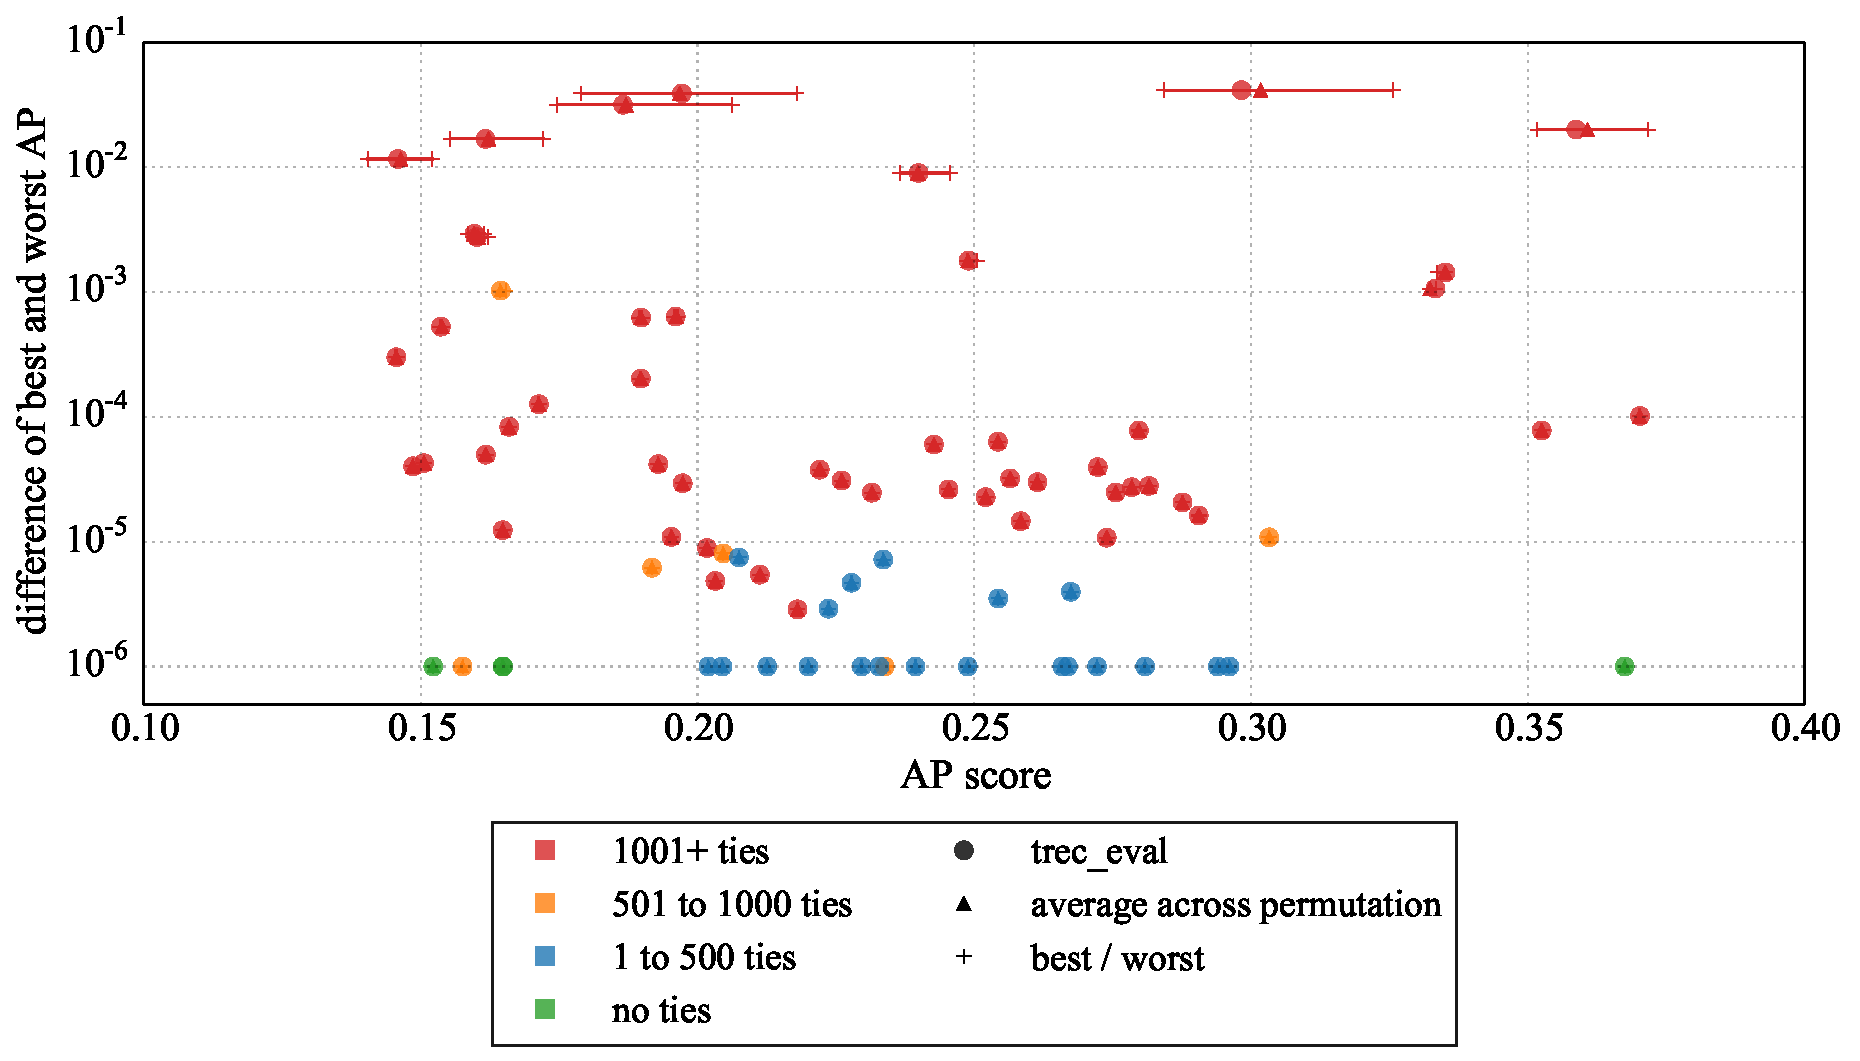
\includegraphics[width=1\textwidth]{figs/fig-trec7-ap-scores.pdf}
\caption{The extent of the imprecision in AP scores arising from ties
in runs.
{\alistair{Need one of the graphs we had many weeks ago, showing that
max score for one system might exceed assigned {\treceval} score for
a supposedly ``better'' system.}}
\label{fig-trec7-ap-scores}}
\end{figure}

Figure~\ref{fig-trec7-ap-scores} plots those $80$ systems.
The horizontal axis is the {\treceval} score for that system,
expressed as a mean AP value over the $50$ topics.
By inspecting the {\treceval} source code we were able to confirm
that it (a) ignored line ordering in the input runs; (b) used
exponential number formats correctly while performing its
sorting-by-score step; and (b) resolved score ties by reverse sorting
on document number, paying no attention to the supplied {\emph{rank}}
field.
The scale on the vertical axis in Figure~\ref{fig-trec7-ap-scores} is
the {\alistair{something}}, meaning that the higher up the scale a
system is plotted, the greater the prevalence of tied scores in its
TREC7 output runs.

Each system is plotted as a multi-point segment.
The left and right ends of the segment reflect the scores that would
be generated by the optimistic and pessimistic orderings with each of
the tied groups; the {\treceval} score is shown as a
{\alistair{diamond?}}, and the ``average across permutations'' score
for that system as a {\alistair{circle?}}.
{\alistair{Get the graph in place, then a few more sentences of
discussion.}}


\myparagraph{Ties in Other Years}

{\alistair{Brief summary (no tables or graphs) of some other TREC
rounds.}}
{\alistair{TREC8: Similar percentages of ties and score/rank
contradictions, and ditto after resorting.}}
